Kapitulu honetan txantiloiaren erabilera landuko da. Txantiloiko berezitasunaz gain, \LaTeX eko elementu nagusiak ere aztertuko dira. 

\section{Txantiloia}

Txantiloian zenbait fitxategi daude. Fitxategi nagusia \texttt{main.tex} izenkoa da. Horrez gain badaude beste fitxategi batzuk \texttt{config} direktorioan. Printzipioz, fitxategi horiek ez dira ikutu behar.

Fitxategi nagusian zenbait atal konfiguratu behar dira.

Lehenik eta behin, txantiloiak \texttt{memoir} estiloa erabiltzen du oinarritzat. Beraz, estilo horretan dauden aukera guztiak erabili daitezke. Gehienbat, \cite{Rmanual} kapituluen itxura alda daiteke estiloak erabiliz. Horretarako, \texttt{main.tex} fitxategiaren hasieran dagoen \texttt{chapterstyle} komandoan estiloa aldatu behar da. Hauek dira aukerak:
\begin{itemize}
	\item bianchi
	\item bringhurst
	\item brotherton
	\item chappell
	\item crosshead
	\item culver
	\item dash
	\item demo2
	\item demo3
	\item dowding
	\item \textbf{ell}
	\item ger
	\item komalike
	\item lyhne
	\item madsen
	\item ntglike
	\item pedersen
	\item \textbf{southall}
	\item \textbf{tandh}
	\item thatcher
	\item veelo
	\item \textbf{verville}
	\item \textbf{wilsondob}
\end{itemize}

Beltzen markatuta dauden estiloetan kapitulu hitza ez da erabiltzen eta, hortaz, euskarazko memorientzako bereziki erabilgarriak dira.

\subsection{Proiektuaren informazioa}

\texttt{information.tex} fitxategian informazio orokorra betetzeko komandoak agertzen dira. Egilearen izena, proiektuaren izenburua, zuzendarien izenak, titulazioa, dokumentuaren data, etab.

\subsection{Dokumentuaren hizkuntza}

Dokumentua euskaraz, gazteleraz edo ingelesez idatzi daiteke. Behar den bezala konfiguratzeko \texttt{main.tex} fitxategian hizkuntza definitu behar da, nahi den aukera deskomentatuz. Bakarrik aukera bat egon behar da deskomentatuta.

\begin{table}[t]
	\centering
	\begin{tabular}{l|llll}
		Y & A & B & C & D\\
		\hline
		y1 & a1 & b1 & c1 & d1\\
		y2 & a2 & b2 & c2 & d2\\
	\end{tabular}
	\caption {Taularen adibidea}\label{tab:adibidea}
\end{table}

\subsection{Dokumentuaren edukia}

Dokumentuaren edukia antolatzeko \texttt{chapters} karpetan dauden fitxategien bidez txertatzen da. \texttt{main.tex} dokumentuan kapituluen ideia garbia izatearren, kapituluen izenburua bertan definitzen da, nahiz eta kodea aipatutako karpetan dauden fitxategien bidez txertatu.


\section{Irudiak eta Taulak}

\begin{figure}[t]
    \centering
	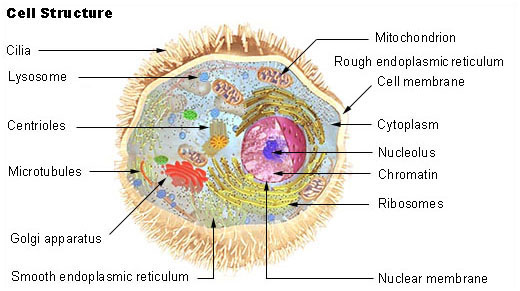
\includegraphics[width=0.75\textwidth]{figures/cell.jpg}
	\caption{Irudiaren adibidea}\label{fig:adibidea}
\end{figure}

Dokumentuaren itxura manentzearren gomendatzen da irudi eta taula guztiak goian edo behan jartzea. Horretarako \texttt{figure} eta \texttt{table} inguruneen \texttt{[t]} edo \texttt{[b]} aukerak erabili behar dira.

\ref{fig:adibidea} irudian eta \ref{tab:adibidea} taulan adibideak ikusi daitezke. Kontutan izan behar da latex sistemak taulen eta irudien kokapen optimoak erabakitzen dituela. Esan bezala, komenigarria da irizpide bat jarraitzea (goian edo behan) eta hori mantentzea. Taula edo irudi baten kokapena orriz aldatzeko, kodearen kokapena aldatu behar da. Kontutan izan irudiaren edo taularen kodea ez daukala zergatik egon aipatzen den tokian, beti zenbakia erabiliz erreferentziatu behar da eta (ez ``goian'' edo ``behan'' terminoak erabiliz).

\section{Algoritmoak eta kode zatiak}

\ref{alg:adibidea} algoritmoan adibidea bat ikusi daiteke.

\clearpage

\begin{algorithm}
\caption{Algoritmo baten adibidea}\label{alg:adibidea}
\begin{algorithmic}
\Require $n \geq 0$
\Ensure $y = x^n$
\State $y \gets 1$
\State $X \gets x$
\State $N \gets n$
\While{$N \neq 0$}
\If{$N$ is even}
    \State $X \gets X \times X$
    \State $N \gets \frac{N}{2}$
\ElsIf{$N$ is odd}
    \State $y \gets y \times X$
    \State $N \gets N - 1$
\EndIf
\EndWhile
\end{algorithmic}
\end{algorithm}

Pakete ugari existitzen dira dokumentuetan kode zatiak txertatzeko. Txantiloi honetan \texttt{lstlisting} paketea erabiltzen da.\footnote{Informazio gehiagorako: \cite{lstlistingdoc}.} Orokorrean, ez da gomendagarria memoriaren gorputzean kodea sartzen, lana ulertzeko ezinbestekoa ez bada. Laukien itxura (koloreak, lerro zenbakiak, etab.) \texttt{config/macros.tex} fitxategian definituta dago. Jarraian kode zati batzuen adibideak erakusten dira. 

Javaz idatzitako kode zatia:

\begin{lstlisting}[language=Java]
public static void main(String args[]) {
    for(int i = 0; i <= 12; i++) { // iruzkina
        System.out.print("12 * "+ i + " = " + 12 * i + "\n");
    }
}
\end{lstlisting}

SQLz idatzitako kode zatia:
\begin{lstlisting}[language=SQL,numbers=none]
select *
from proiektuak
where nota between 8 and 10
\end{lstlisting}


\section{Erreferentziak}

Bibliografia sartzeko BibTeX erabili behar da. Erreferntziak \texttt{references.bib} fitxategian daude, eta textuan errferenziatzeko \texttt{cite} komandoa erabili behar da. Adibidez, \cite{Shahbaba2011} edo \cite{Efron1994, Rmanual, Subramanian2005gene}. Ez ahaztu erreferentzien informazio guztia sartzen (orrialdeak, urtea, etab.).

